% mycsrf 'for beeing included' snippet template
%
% (c) Karsten Reincke, Frankfurt a.M. 2012, ff.
%
% This text is licensed under the Creative Commons Attribution 3.0 Germany
% License (http://creativecommons.org/licenses/by/3.0/de/): Feel free to share
% (to copy, distribute and transmit) or to remix (to adapt) it, if you respect
% how you must attribute the work in the manner specified by the author(s):
% \newline
% In an internet based reuse please link the reused parts to mycsrf.fodina.de
% and mention the original author Karsten Reincke in a suitable manner. In a
% paper-like reuse please insert a short hint to mycsrf.fodina.de and to the
% original author, Karsten Reincke, into your preface. For normal quotations
% please use the scientific standard to cite

%% use all entries of the bibliography
\subsection{PMX (und M-TX): die Nicht-Vereinfachung ($\bigstar\bigstar$)}

\subsubsection{Das große Versprechen: Kadenz I und III}

Wer MusiX\TeX\ nutzt, dem drängt sich immer wieder einmal der Gedanke auf, dass
das doch auch einfacher gehen müsste. Und in der Tat: Legt man für die vielen
Kleinigkeiten, mit denen man bei MusiX\TeX\ jeden Einzelfall gestalten darf, ein
paar Standards fest, sollte man eine einfachere Sprache 'erfinden' können. Mit
der würde man seine Notentexte formulieren. Und das Ergebnis würde zuletzt
maschinell wieder in MusiX\TeX-Code übersetzt werden. Genau das ist der
Grundgedanke von \textit{PMX}\footnote{\cite[vgl.][\nopage wp]{CtanPmx2018a}.
Diese Paketbeschreibung gibt an, dass \acc{PMX} unter der GPL-2.0
distribuiert wird. Das ist eine anerkannte Open-Source-Lizenz ($\rightarrow$
\href{https://opensource.org/licenses/GPL-2.0}
{https://opensource.org/licenses/GPL-2.0}).}, einem Präprozessor für
MusiX\TeX.\footcite[Vgl.][4ff]{CtanPmx2018a}

Ein \textit{PMX}-Tutorial nennt MusiX\TeX\ eines der besten Programme für den
elektronischen Notensatz.\footcite[vgl][2]{Noack2013a} Allerdings habe es ein
nicht eben intuitives 'Look and Feel', biete kein 'WYSIWYG' und könne ob seiner
Natur als symbolische Auszeichnungssprache (nicht nur Musiker)
entmutigen\footcite[vgl][2]{Noack2013a}: Selbst nach einer sorgfältigen und
sauberen Installation bleibe das Setzen einer Partitur ein mühsames
Unterfangen.\footcite[vgl][3]{Noack2013a}

Einen Ausweg aus diesem Dilemma -- so das Tutorial -- biete \textit{PMX}, das als
Präprozessor den Eingabeprozess dramatisch vereinfache und so etwas liefere, was
zu den einfachsten Möglichkeiten gehöre, Notenblätter elektronisch zu
erarbeiten.\footcite[vgl][3]{Noack2013a} Die Gegenüberstellung der
MusiX\TeX-Variante und der PMX-Variante derselben Noten unterstreicht diese
vollmundigen Ankündigungen.\footcite[vgl][3]{Noack2013a}

Betrachtet man die Sache logisch, ist die Emphase nicht unangemessen: Es gehört
zum Wesen eines Präprozessors, dass er einen (meist) vereinfachten Code nimmt
und auf die (meist) komplexere und kompliziertere Hauptsprache abbildet. Das
hieße in diesem Fall, dass die herausragenden typographischen Fähigkeiten von
MusiX\TeX\ erhalten blieben, ohne dass man weiterhin seine überbordende
Syntagmen zu tippen hätte. Und dass dem tatsächlich so ist, können auch wir an
unser kleinen Grabner-Kadenz\footcite[vgl.][107]{Grabner1974a} demonstrieren:

\begin{center}
\includegraphics{pics/pmx/cadenca1}
\cad{I}{PMX}
\end{center}

Der entsprechende kommentierte PMX-Code sieht so aus:
\begin{verbatim}
%%% PREAMBLE; %%%%%%%%%%%%%%%%%%%%%%%%%%%%%%%%%%%%%%%%%%%%%%%%%%%%%%%
% nstaves | ninstr | mtrnuml  | mtrdenl | mtrnump | mtrdenp | npickup
     1        1        3           0         0         0         0
%  nkeys  | npages | nsystems | musicsize | fracident
     0        0         4         16           .0
% no instrument name = blank line

% tremble
t
./
% BODY: HEADER: a smaller width than the line width
w80m
%%% MUSIC: %%%%%%%%%%%%%%%%%%%%%%%%%%%%%%%%%%%%%%%%
\zcharnote{-10}{I}\  \zcharnote{+10}{T}\ c04 ze zg 
\zcharnote{-10}{IV}\ \zcharnote{+10}{S}\ f04 za zc 
\zcharnote{-10}{V}\  \zcharnote{+10}{D}\ g04 zb zd
| 
\zcharnote{-10}{I}\  \zcharnote{+10}{T}\ a03 zc ze 
\zcharnote{-10}{IV}\ \zcharnote{+10}{S}\ d04 zf za
\zcharnote{-10}{V}\  \zcharnote{+10}{D}\ e04 zgs zb
%%%%%%%%%%%%%%%%%%%%%%%%%%%%%%%%%%%%%%%%%%%%%%%% EOF
\end{verbatim}

Man erkennt, dass sich das Handling der Notenbezeichnungen gegenüber dem
MusiX\TeX-Sourcetext verschlankt hat. Noch auffälliger wird das bei unser
dritten Referenzkadenz:
\begin{center}
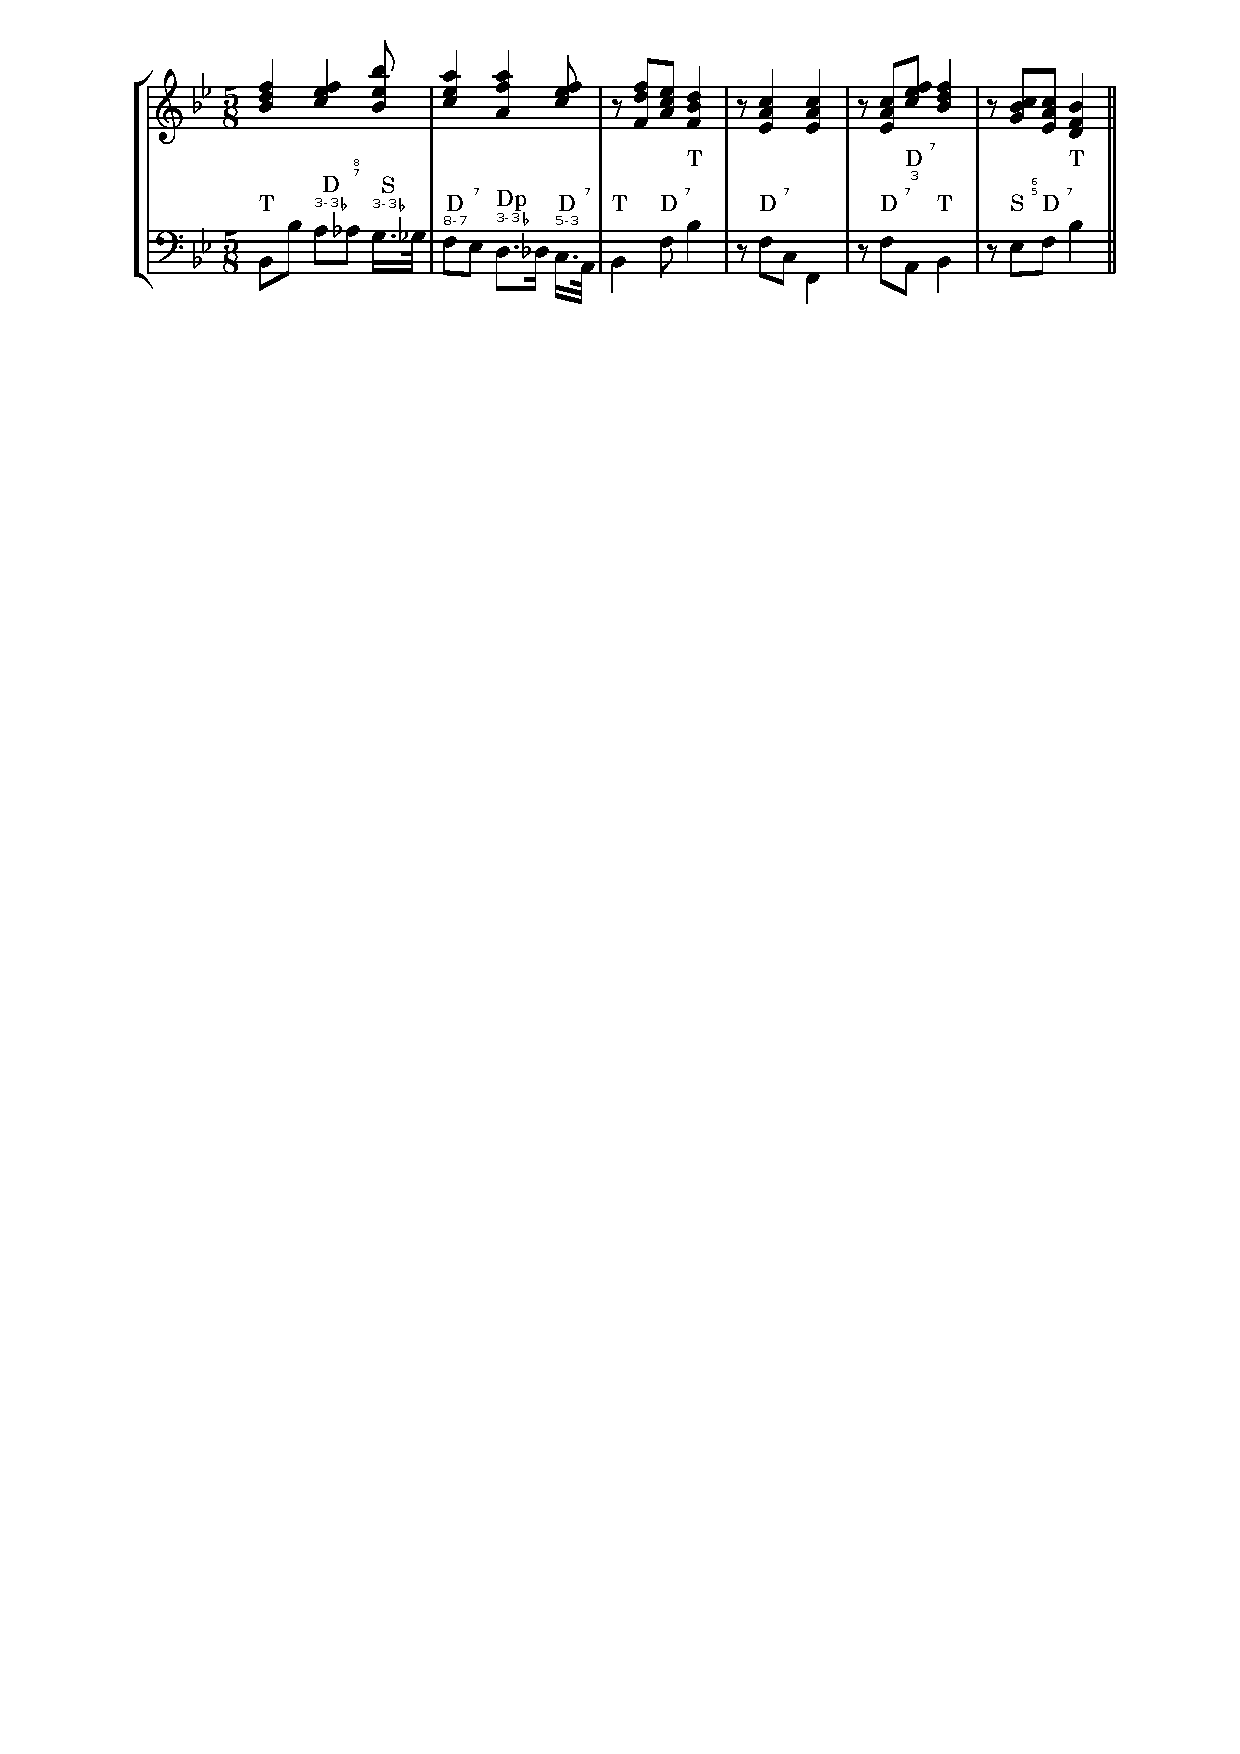
\includegraphics{pics/pmx/cadenca3}
\cad{III}{PMX}
\end{center}

Zu ihr gehört dieser Sourcecode:

\begin{verbatim}
%%% PREAMBLE: %%%%%%%%%%%%%%%%%%%%%%%%%%%%%%%%%%%%%%%%%%%%%%%%%%%%%%%
% nstaves | ninstr | mtrnuml  | mtrdenl | mtrnump | mtrdenp | npickup
     2        2         5          8         5         8         0
%  nkeys  | npages | nsystems | musicsize | fracident
     -2        0         3          16          .1
Bass
Diskant
bt
./
%%% BODY: %%%%%%%%%%%%%%%%%%%%%%%%%%%%%%%%%%%%%%%%%%%%%%%%%%%%%%%%%%% 
%%% HEADER: %%%%%%%%%%%%%%%%%%%%%%%%%%%%%%%%%%%%%%%%%%%%%%%%%%%%%%%%% 
\\font\ref=cmr10\def\zt#1#2{\zcharnote{#1}{\ref#2}}\def\bs{$\backslash$}\
%a smaller width than the line width
w130m
%%% MUSIC: %%%%%%%%%%%%%%%%%%%%%%%%%%%%%%%%%%%%%%%%%%%%%%%%%%%%%%%%%%%
%%% T1: %%%%%%%%%%%%%%%%%%%%%%%%%%%%%%%%%%%%%
[l b82 b8+ ] [l a8 a8f ] [l g1d g3 ] |/
\zt{-7}{T}\  b44u zd zf 
\zt{-7}{D7}\ cu ze zf 
\zt{-7}{S}\  b8-u ze zb+ |/
%%% T2: %%%%%%%%%%%%%%%%%%%%%%%%%%%%%%%%%%%%%
 [l f83 e83 ] [l d83d d13f ] [l c13d a32 ] |/
\zt{-7}{D7}\ c4-u ze za
\zt{-7}{Dp}\ a-u zd za+ 
\zt{-7}{D7}\ c8-u ze zf   |/
%%% T3: %%%%%%%%%%%%%%%%%%%%%%%%%%%%%%%%%%%%%
b42 f83 b43 |/
r8 \zt{-7}{T}\  [uh f85 zd zf-
   \zt{-7}{D7}\ e85 zc za ] 
   \zt{-7}{T}\  d4- zf zb |/
%%% T4: %%%%%%%%%%%%%%%%%%%%%%%%%%%%%%%%%%%%%
r8 f83 c83 f42 |/
r8 \zt{-7}{D7}\ e44 za zc e44 za zc |/
%%% T5: %%%%%%%%%%%%%%%%%%%%%%%%%%%%%%%%%%%%%
r8 [l f83 a8- ] b42l |/
r8 \zt{-7}{D7}\ [u c85 za ze c85 ze zf ] 
   \zt{-7}{T}\   b44u zf+ zd |/
%%% T6: %%%%%%%%%%%%%%%%%%%%%%%%%%%%%%%%%%%%%%
r8 [l e83 f8 ] b4l |/
r8 \zt{-7}{D7}\ [u c85 zb zg c85 za ze ] 
   \zt{-7}{T}\ b44u zf zd |/
%%%%%%%%%%%%%%%%%%%%%%%%%%%%%%%%%%%%%%%%%%% EOF
\end{verbatim}

Schon der erste Akkord aus der Musix\TeX-Variante
\begin{center}\texttt{\textbackslash{NOtes}
\textbackslash{Dqbl} I b \&
\textbackslash{zq}\{ik\}\textbackslash{qu}\{m\} \textbackslash{en}} \end{center}
reduziert\footnote{Um mal die reinen Notensymbole gegenüberzustellen, haben wir
diesmal die in beiden Varianten als \TeX-Code integrierten Analysesymbole
weggelassen.} sich zum schlichteren
\begin{center}\texttt{[l b82 b8+ ] |/ b44u zd zf }\end{center}

\subsubsection{\ldots der Wermutstropfen \ldots}

Trotz der so euphorisch kolportierten Vorteile wächst sich \textit{PMX} bei
näherem Hinsehen für den Musikwissenschaftler zu einer Enttäuschung aus.
Gehen wir die Punkte der Reihe nach durch:

\paragraph{\small Inkompatibilitäten}$\;$ \\

Zunächst müssen wir 'gestehen', dass wir in diesem Kapitel unseres
'selbstreferentiellen' Dokumentes bei der Gegenüberstellung von Notentext und
generierendem Code 'geschummelt' haben: Es gibt überhaupt keine Möglichkeit,
PMX-Code in \LaTeX-Code einzubetten und daraus dann -- sozusagen in einem Rutsch
-- eine PDF-Datei zu erzeugen.
Das liegt in erster Linie an der Arbeitsweise von \textit{PMX}\footnote{In zweiter
Linie liegt es an den Entwicklern von \textit{PMX}. Sie haben schlicht (noch) kein
korrespondierendes \LaTeX-Paket geschaffen. Technisch mag das herausfordernd
sein, unmöglich ist es nicht: Es wird ja schon gesagt, dass der von \textit{pmxab}
erzeugte Code eigentlich 'nur' auf die richtige Weise auskommentiert werden
müsse, damit er in der \texttt{\textbackslash{begin/end}\{music\}}-Umgebung
genutzt werden könne (\cite[vgl.][94]{Noack2013a}). Mithin sollte der Schritt zu
einer integrierten Lösung so groß nicht sein.}: Als Päprozessor nimmt das
entsprechende Tool \textit{pmxab} eine \textit{PMX}-Datei und erzeugt daraus eine
MusiX\TeX-Datei. Diese MusiX\TeX-Datei ist von ihrem Dialekt her aber eine
vollständige MusiX\TeX-Datei und kein inkludierbares Code-Snippet, das 1:1 in die
\LaTeX-Umgebung
\texttt{\textbackslash{begin}\{music\} \ldots \textbackslash{end}\{music\}}
eingebettet werden könnte. Entsprechende Versuche müssen scheitern.


\begin{verbbox}[\footnotesize]
.pmx.eps:
  @ make \$< `basename \$< .pmx`.tex
  @ musixtex -g `basename \$< .pmx`.tex
  @ ps2eps `basename \$< .pmx`.ps
.pmx.tex:
   @ pmxab \$<
\end{verbbox}

\label{PmxGraphics} Die eine, 'direkte' Lösung für dieses Problem besteht darin,
zuerst -- ganz \LaTeX-unabhängig -- aus der \textit{PMX}-Datei eine Graphik zu
erzeugen und diese anschließend in die \LaTeX-Datei einzubinden\footcite[Vgl.
dazu auch][94]{Noack2013a}:

\begin{itemize}
  \item Dazu ruft man für eine \textit{PMX}-Datei zunächst den
  \textit{PMX}-Präprozessor auf (z.B. \texttt{pmxab candeza1.pmx}), um die
  korrespondierende MusiX\TeX-Datei \texttt{candeza1.tex} zu genieren.
  \item Das Resultat übergibt man dann dem \textit{MusiX\TeX}-Tool als Input, und
  zwar mit der Option \textit{-g}: (\texttt{musixtex -g candeza1.tex}). So wird
  nicht eine \textit{PDF}-Datei erzeugt, sondern die Postscriptdatei
  \texttt{candeza1.ps}.
  \item Danach lässt man diese Postscriptdatei in eine 
  Encapsulated-Postscript-Datei umwandeln (\texttt{ps2eps
  candeza1.ps}).\footnote{Eine make-basierte
  Automatisierung dieser Schritte enthielte als Kern wohl dies:\vspace{0.2em}\\
  \theverbbox\ \vspace{0.2em}\\
  \cite[Vgl. dazu][\nopage Makefile aus dem Verzeichnis 'pmx']{Reincke2019a}.}
  \item Und ganz zuletzt fügt man an der Stelle der \LaTeX-Datei, wo die
  \textit{eps}-Graphik erscheinen soll, den \LaTeX-Befehl 
  \texttt{\textbackslash{includegraphics}\{candeza1.eps\}}
  ein\footnote{Hier muss man beachten, an der Stelle, von wo aus man die
  \textit{eps}-Datei einlesen will, nicht (versehentlich) auch eine 'gleichnamige'
  \textit{pdf}-Datei abgelegt zu haben. In diesem Fall lädt
  \texttt{includegraphix} nämlich letztere. Und das wird im \LaTeX-Dokument zu
  unerwarteten Seitenumbrüchen führen, nach deren Ursache man u.U. lange sucht.
  }
\end{itemize}

Diese Umstände müssen -- wenigstens den Musikwissenschaftler -- enttäuschen:
Wenn man zuletzt doch eine Graphik einbindet, die man mit einem externen Tool
erstellt hat, warum sollte man sich dann die Mühe antun, zwecks Erstellung einer
Graphik zuerst \textit{PMX} zu lernen, wo es doch so viele gute
Notensatzprogramme gibt, die ihre Daten -- auch ohne Umweg über Shellkommandos
-- als Postscript- oder PDF-Datei exportieren?\footnote{Zu Erinnerung:
\textit{ABC} geht implizit genauso vor.
Insofern träfe dieses Argument eben auch \textit{ABC}. Allerdings punktet
\textit{ABC} durch seine vielen Konverter und Tools und durch seine lange
Tradition.} Das könnte doch nur dann sinnvoll sein, wenn man wenigstens auf die
gestalterischen Vorzüge und Freiheiten von MusiX\TeX\ zugreifen könnte. Aber
nicht einmal das ist ja der Fall -- wie wir gleich sehen werden.

Zunächst müssen wir aber der Wahrheit Genüge tun und darauf hinweisen, dass der
Autor des \textit{PMX}-Tutorials die Irritationen in Sachen \textit{PMX /
MusiX\TeX}\ und \textit{\LaTeX}\ kennt und auch anspricht: Seinem eigenen
Bekunden nach würde beide Ansätze konkurrierend und überschneidend das Layout
gestalten und viel Spezialbefehle zueinander inkompatibel definieren, unabhängig
davon, dass sie bei auf \TeX\ aufsetzen.\footcite[vgl.][93]{Noack2013a} Und so
kommt er zu dem Schluss:

\begin{quote}\textit{\enquote{While with modern implementations of ressources
are no longer a serious problem, the incompatibility problems are, and their
resolution would be a major programming task. So there have, to this day, not
been any serious efforts to provide a truly merged version of \LaTeX\ with
PMX.}\footnote{\cite[vgl.][93f]{Noack2013a}. Man muss an dieser Stelle auch
im Kopf behalten, dass PMX nicht für die Nutzung in \LaTeX\ entwickelt worden ist.
Es ging den Entwicklern darum, besser und einfacher qualitativ hochwertige
Notenblätter zu erzeugen. Und für diesen Zweck ist die Lösung \textit{PMX
/ MusiX\TeX} sehr wohl geeignet. Nur ist die Gestaltung solcher Blätter meist nicht
Aufgabe von Musikwissenschaftlern.}
}\end{quote}

Verwendet man \acc{PMX} trotzdem, bleiben zuletzt doch noch Wünche offen:

\paragraph{\small Unzulänglichkeiten}$\;$ \\

Die erste kleinere Unzulänglichkeit betrifft das Erscheinungsbild: Die
Kadenz-III in der \textit{PMX}-Variante\footnote{$\rightarrow$ S.
\pageref{\cadlab{III}{PMX}}} wirkt optisch weniger klar als die
\textit{MusiX\TeX}-Variante.\footnote{$\rightarrow$ S.
\pageref{\cadlab{III}{MusiXTeX}}} Dies liegt am 5/8-Takt. Der kann in eine 3er-
und eine 2er Hälfte oder in eine 2er und eine 3er Hälfte aufgeteilt werden. Und
das 3. Achtel der 3er-Hälfte kann auftaktisch gemeint sein. Die Entscheidungen,
die \textit{PMX} -- sozusagen nach Schema F -- automatisch trifft, werden solchen
kontextbedingten Feinheiten nicht gerecht.\footnote{Gelegentlich wird
man diese allerdings auch für reine Geschmacksfragen halten dürfen.}

Die zweite Unzulänglichkeit betrifft die Methode, wie die Analysesymbole in den
\textit{PMX}-Code eingettet werden: \textit{PMX} bietet zwar die Möglichkeit, Stücke
auf \textit{PMX}-Level textuell zu kennzeichnen oder Texte über oder unter den
Systemen einzufügen.\footcite[vgl.][61f]{Noack2013a} Wenn es aber -- wie bei der
Musikwissenschaft notwendig -- darum geht, Symbole und Texte graphisch variabel
einzufügen, dann muss der \textit{PMX}-User auf \enquote{Inline \TeX\ commands}
zurückgreifen, also unter den \LaTeX-Level auf den \TeX-Level
'zurückfallen'\footcite[vgl.][76f]{Noack2013a}: die Nutzung einer vereinfachten
\textit{PMX}-Syntax wird dann um den Preis einer komplizierten Eingabe von
\TeX-Syntagmen erkauft.\footnote{Weil \TeX\ 'zu' kompliziert war, wurde \LaTeX\
'erfunden'; und weil \textit{PMX} mit Liedtext 'zu' kompliziert war, entstand
\textit{M-Tx} (\cite[vgl.][\nopage wp]{CtanMtx2018a}) -- einschließlich eines
Handbuches (\cite[vgl.][3ff]{Laurie2017a})}

Wirklich unzulänglich ist dabei jedoch das, \textit{was} eingebettet werden
kann. Was schon bei den ABC-Lösungen galt\footnote{$\rightarrow$ S.
\pageref{AppraisalABC}}, trifft auch hier zu: Aus der \LaTeX-Welt können weder
hoch- und/oder tiefgestellte Kleinsymbole oder Sonderzeichen eingefügt werden,
noch die Alterationszeichen $\sharp$, $\flat$ oder $\natural$ aus den
Sonderzeichen - ganz zu schweigen von der Einbettung jener ausgefeilten
Konstrukte, die das \textit{harmony}-Paket zur Verfügung stellt. Denn das
Konvertierungstool \textit{pmxab}, das \textit{MusiX\TeX}-Code aus
\textit{PMX}-Code ableitet, arbeitet ja noch außerhalb von \TeX. Und das
Konvertierungstool \textit{musixtex} versteht 'nur' \textit{Musix\TeX}-Code,
nicht aber \LaTeX-Syntagmen.

\subsubsection{\ldots und die kleine Lösung: Kadenz II}

Trotz all dieser Nicklichkeiten kann es für den Musikwissenschaftler
gelegentlich sehr wohl Sinn machen, im Kontext einer \LaTeX-Arbeit\footnote{mit
inkludiertem MusiX\TeX-Package} auf \textit{PMX} zurückzugreifen: Wenn es nämlich
gilt, viele längere Musikbeispiele zu verwenden, wird das manuelle Tippen des
MusiX\TeX-Codes zu einer langwierigen, fehlerträchtigen Angelegenheit werden.

Eine Lösung dafür bestünde darin, zuerst den reinen Notentext mit \textit{PMX} zu
erstellen und dann mit \textit{pmxab} in MusiX\TeX-Code umzuwandeln. Danach griffe
man auf die Option zurück, -- wie im Tutorial als Möglichkeit angedeutet --
\enquote{manuell} bestimmte Zeilen des automatisch generierten Codes
auszukommentieren und so etwas zu erzeugen, was tatsächlich in die
\verb|\begin{music}...\end{music}|-\LaTeX-Umgebung kopiert werden
kann.\footcite[vgl.][94]{Noack2013a} Dieses Verfahren wollen wir noch kurz
vorführen:

Wir wissen ja schon, dass wir die (beschränkten) Symbole der Harmonieanalyse,
die wir auf \textit{PMX}-Level einzugeben vermögen, bei einer Einbettung in
einen \LaTeX-Code werden nicht verwenden können, eben weil es ja keine
\LaTeX-Konstrukte sind, sondern \TeX-Syntagmen. Deshalb notieren wir diesmal auf
\textit{PMX}-Level nur den Notentext. Das 'reine' PMX/MusiX\TeX-Verfahren würde
daraus die folgende Graphik erzeugen:\footnote{PMX-Code $\rightarrow$
\texttt{pmxab} $\rightarrow$ Musix\TeX-Code $\rightarrow$ \texttt{musictex -g} 
$\rightarrow$ PS-Code  $\rightarrow$ \texttt{ps2eps} $\rightarrow$ EPS-Graphik }


\begin{center}
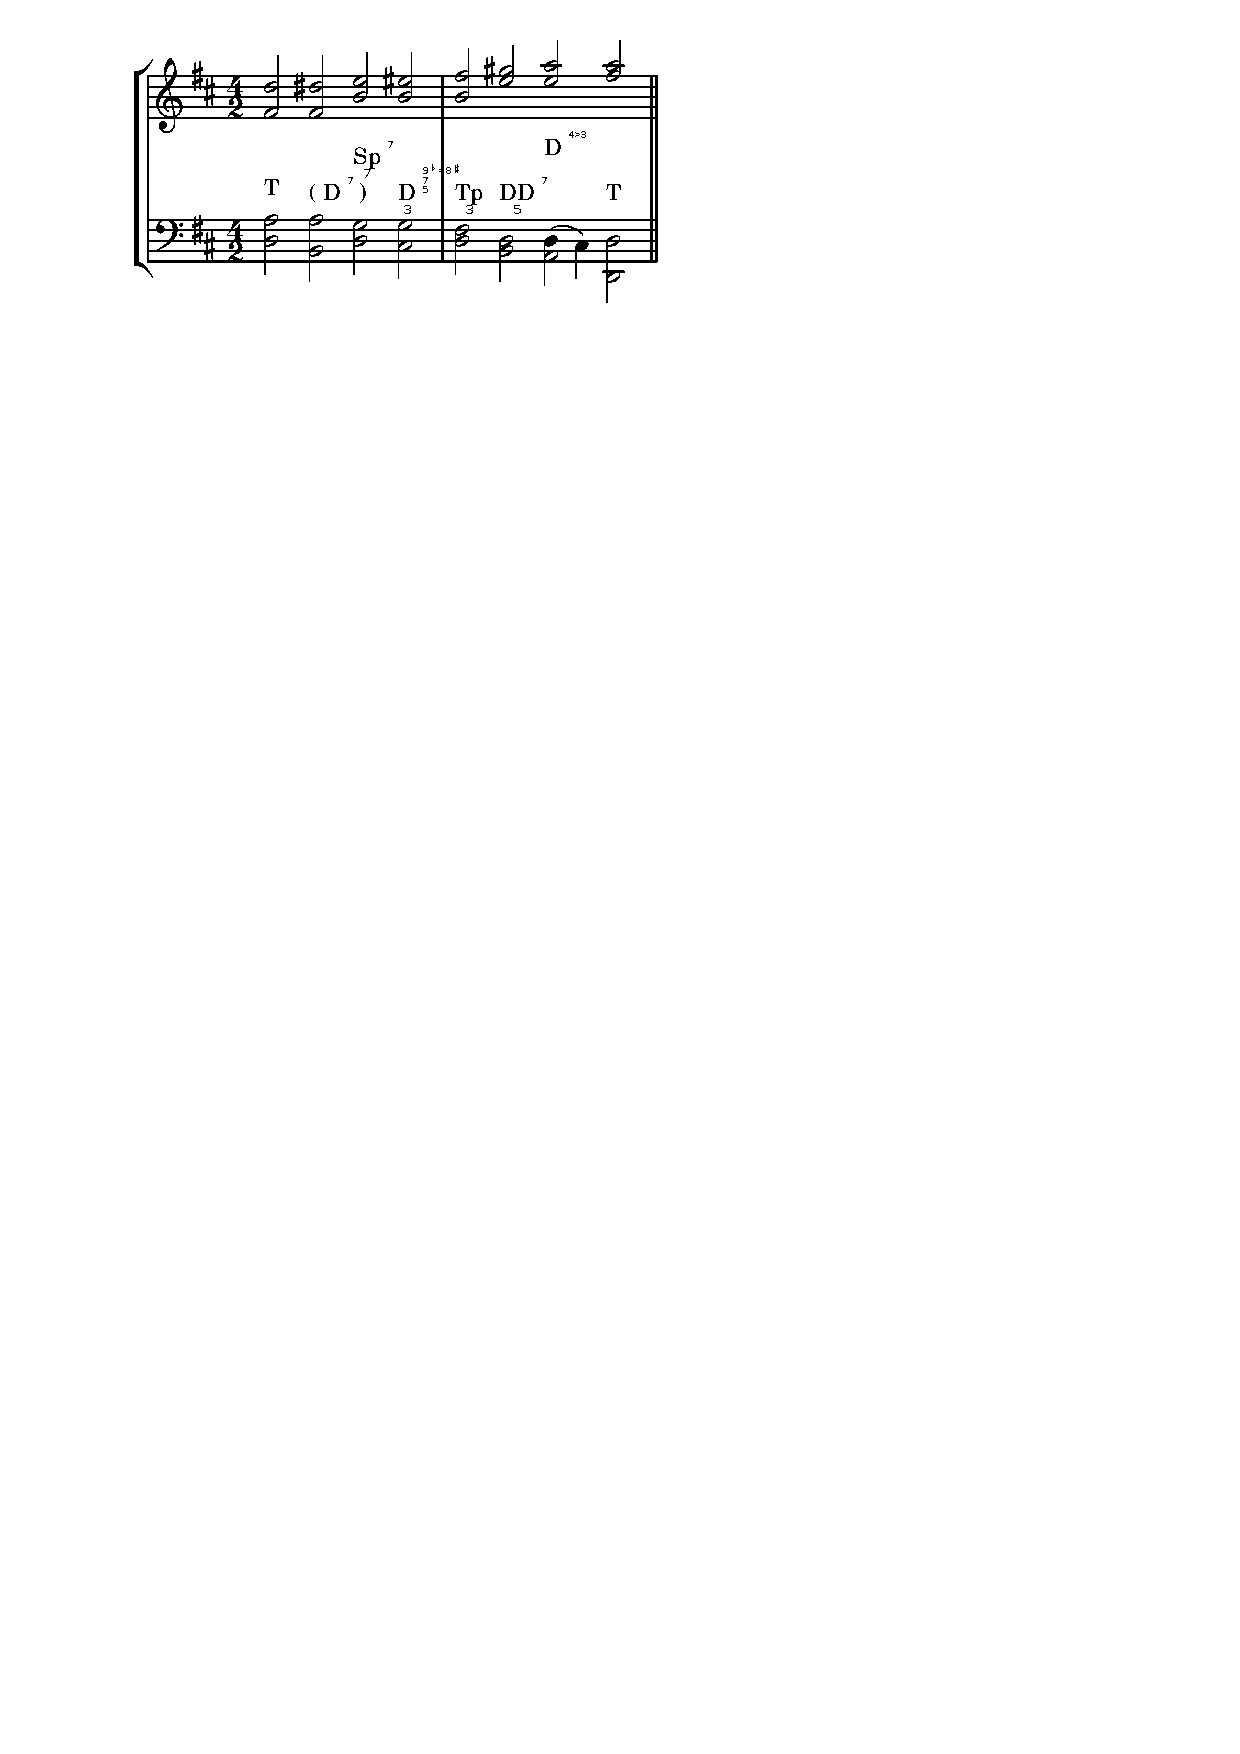
\includegraphics{pics/pmx/cadenca2}
\cad{II}{PMX}
\end{center}

Ausgegangen wird dabei von folgendem \textit{PMX}-Code:

\begin{verbatim}
% PREAMBLE %%%%%%%%%%%%%%%%%%%%%%%%%%%%%%%%%%%%%%%%%%%%%%%%%%%%%%%%%%
% nstaves | ninstr | mtrnuml  | mtrdenl | mtrnump | mtrdenp | npickup
     2        1         4          2         4         2         0
%  nkeys  | npages | nsystems | musicsize | fracident
     2        0         3          16          .1
Piano
bt
./
% BODY: %%%%%%%%%%%%%%%%%%%%%%%%%%%%%%%%%%%%%%%%%%%%%%%%%%%%%%%%%%%%%
% HEADER: %%%%%%%%%%%%%%%%%%%%%%%%%%%%%%%%%%%%%%%%
%a smaller width than the line width
w130m
% MUSIC: %%%%%%%%%%%%%%%%%%%%%%%%%%%%%%%%%%%%%%%%%
% T:1-1     T:1-2    T:1-3                T:1-4
  d23l za+  b-l za+  d-l zg              c-l zg+ |/
  f24u zd+  f-u zd+s  bu  ze              bu zes |/
% %%%%%%%%%%%%%%%%%%%%%%%%%%%%%%%%%%%%%%%%%%%%%%%%%
% T:2-1     T:2-2    T:2-3                T:2-4
  d23l zf  b-l  zd   (u d4 za2 c4 za2 )   d2-l zd+  /
  b24u zf+  e  zgs   e  za                f  za |/
% %%%%%%%%%%%%%%%%%%%%%%%%%%%%%%%%%%%%%%%%%%%%%  EOF 
\end{verbatim}

Lässt man diesen \textit{PMX}-Code von \texttt{pmxab} verarbeiten, entsteht ein
Musix\TeX-Code, bei dem man, will man ihn erfolgreich in eine
Musix\TeX-in-\LaTeX-Umgebung \verb|\begin{music}| ... \verb|\\end{music}|
einbetten, noch  einige Zeilen auskommentieren und einige Werte ändern muss:

\begin{verbatim}
\begin{music}
%%ignore:%% \input musixtex
%%ignore:%% \input pmx
%%ignore:%% \setmaxslurs{24}\setmaxinstruments{24}%
\normalmusicsize %%% instead of: %%% \smallmusicsize%
%%ignore:%% \nopagenumbers
%%ignore:%% \tracingstats=2\relax
%%ignore:%% \hsize=369pt
%%ignore:%% \vsize740pt
\def\nbinstruments{1}
\setstaffs12
\setclef1{60}
\setname1{Piano}
\generalsignature{ 2}%
\generalmeter{\meterfrac{4}{2}}%
\parindent 4em %%% instead of %%% 37pt
%%ignore:%% \elemskip1pt\afterruleskip1.000pt\beforeruleskip0pt\relax
%%ignore:%% \stafftopmarg0pt\staffbotmarg5\Interligne\interstaff{10}\relax
%%ignore:%% \readmod{cadenca2}
%%ignore:%% \startmuflex
\startpiece
%%ignore:%% \addspace
%%ignore:%% \afterruleskip%
%%ignore:%% \znotes|\zcharnote{16}{\titles{2.0}{}{0}{}{0}{}{0}}\en%
% Bar count 1
\pnotes{4.00}\zh{''A}\hl{`D}\zh{'A}\hl{`B}\zh G\hl D\zh G\hl C|\zh{'d}%
\hu{`f}\bigsh{'d}\zh d\hu{`f}\zh{'e}\hu b\bigsh e\zh e\hu b\en%
% Bar count 2
\xbar
\pnotes{4.00}\zh{'F}\hl D\zh D\hl B|\zh{'f}\hu b\bigsh g\zh g\hl e\en%
\pnotes{2.83}\zq A\qu D \zq A\qu C|\zh{''a}\hl{`e}%
%%ignore: \isu0{'D}{.8} \tslur0A
\en%
\pnotes{4.00}\zh{'D}\hl{`D}|\zh{''a}\hl{`f}\en%
\Endpiece
%%ignore:%% \vfill\eject\endmuflex
%%ignore:%% \bye
\end{music}%
\end{verbatim}

Vor einer erfolgreichen Nutzung diese Codes muss man in seinem \LaTeX-Header
außerdem noch die Regel \verb|\newcommand{\pnotes}[1]{\notes}| formuliert haben,
damit aus der Einbettung auf \LaTeX/MusiX\TeX-Ebene -- also ohne Einbindung
einer externen Graphik -- das folgende Bild  entsteht:

\vspace{0.7cm}
\begin{music}
%%ignore:%% \input musixtex
%%ignore:%% \input pmx
%%ignore:%% \setmaxslurs{24}\setmaxinstruments{24}%
\normalmusicsize %%% instead of: %%% \smallmusicsize%
%%ignore:%% \nopagenumbers
%%ignore:%% \tracingstats=2\relax
%%ignore:%% \hsize=369pt
%%ignore:%% \vsize740pt
\def\nbinstruments{1}
\setstaffs12
\setclef1{60}
\setname1{Piano}
\generalsignature{ 2}%
\generalmeter{\meterfrac{4}{2}}%
\parindent 4em %%% instead of %%% 37pt
%%ignore:%% \elemskip1pt\afterruleskip1.000pt\beforeruleskip0pt\relax
%%ignore:%% \stafftopmarg0pt\staffbotmarg5\Interligne\interstaff{10}\relax
%%ignore:%% \readmod{cadenca2}
%%ignore:%% \startmuflex
\startpiece
%%ignore:%% \addspace
%%ignore:%% \afterruleskip%
%%ignore:%% \znotes|\zcharnote{16}{\titles{2.0}{}{0}{}{0}{}{0}}\en%
% Bar count 1
\pnotes{4.00}\zh{''A}\hl{`D}\zh{'A}\hl{`B}\zh G\hl D\zh G\hl C|\zh{'d}%
\hu{`f}\bigsh{'d}\zh d\hu{`f}\zh{'e}\hu b\bigsh e\zh e\hu b\en%
% Bar count 2
\xbar
\pnotes{4.00}\zh{'F}\hl D\zh D\hl B|\zh{'f}\hu b\bigsh g\zh g\hl e\en%
\pnotes{2.83}\zq A\qu D \zq A\qu C|\zh{''a}\hl{`e}%
%%ignore: \isu0{'D}{.8} \tslur0A
\en%
\pnotes{4.00}\zh{'D}\hl{`D}|\zh{''a}\hl{`f}\en%
\Endpiece
%%ignore:%% \vfill\eject\endmuflex
%%ignore:%% \bye
\end{music}%
\cad{II}{PMX+MusiXTeX-in-LaTeX}
\vspace{0.7cm}

An dieser Version erkennt man jedoch auch, dass die Vorstellung, man brauche
bloß mal eben Zeilen auszukommentieren, der Sachlage nicht gerecht wird: Damit
obiger Code überhaupt kompilierbar wurde, mussten wir die Vorhaltsklammer im
Bass aus dem Code herausnehmen, was dort unmittelbar zu einer ungewollten
Oktavierung führte. Tatsächlich wird man -- falls man den MusiX\TeX-Code in
seinen \LaTeX-Code einfügen will, den \texttt{pmxab} aus der \textit{pmx}-Datei
erzeugt -- ein wenig 'Tuning'-Zeit einplanen müssen. Geht man diesen Weg, kann
man allerdings auch die \LaTeX-basierten Elemente einer Harmonieanalyse
darin verwenden. Man hat also in der Tat die gestalterische Freiheit auf
\LaTeX-MusiX\TeX-Level gewonnen, ohne den komplexen und komplizierten
MusiX\TeX-Code als Ganzes selbst entworfen haben zu müssen. Die Grundarbeit
erledigt man auf \textit{PMX}-Level, die Feinheiten fügt man manuell ein:

\vspace{0.7cm}
\begin{music}%
\normalmusicsize %%% instead of: %%% \smallmusicsize%
\def\nbinstruments{1}
\setstaffs12
\setclef1{60}
\setname1{Piano}
\generalsignature{ 2}%
\generalmeter{\meterfrac{4}{2}}%
\parindent 4em %%% instead of %%% 37pt
\startpiece
% Bar count 1
\notes
  \zmidstaff{\HH.T.....}\zh{''A}\hl{`D}%
  \zmidstaff{(\HH.D..7...)}\zh{'A}\hl{`B}%
  \zmidstaff{\HH.Sp.7...7.}\zh G\hl D
  \zmidstaff{\HH.\Dohne.3.$\flat$9=$\sharp$8.7.5.}\zh G\hl C |%
  \zh{'d}\hu{`f}\bigsh{'d}\zh d\hu{`f}%
  \zh{'e}\hu b\bigsh{e}\zh e\hu b%
\en%
% Bar count 2
\xbar
\notes
  \zmidstaff{\HH.Tp.3....}\zh{'F}\hl D%
  \zmidstaff{\HH.\DD.5...7.}\zh D\hl B |%
  \zh{'f}\hu b\bigsh g%
  \zh g\hl e%
\en%
\notes
  \zmidstaff{\HH.D....4-3.}%
  \zh{H}\isluru{0}{K}\qu{K}\tslur{0}{J}\qu{J}|%
  \zh{''a}\hl{`e}%
\en%
\notes
  \zmidstaff{\HH.T.....}\zh{'D}\hl{`D}  |%
  \zh{''a}\hl{`f}%
\en%
\Endpiece
\end{music}%
\cad{II}{PMX+MusiXTeX-in-LaTeX++}
\vspace{0.7cm}
 
Hilfreich sind dabei -- zugegebenermaßen -- Geduld, ein geschulter Blick und der
Wille zum 'Codeclearing':

\begin{verbatim}
\begin{music}%
\normalmusicsize %%% instead of: %%% \smallmusicsize%
\def\nbinstruments{1}
\setstaffs12
\setclef1{60}
\setname1{Piano}
\generalsignature{ 2}%
\generalmeter{\meterfrac{4}{2}}%
\parindent 4em %%% instead of %%% 37pt
\startpiece
% Bar count 1
\notes
  \zmidstaff{\HH.T.....}\zh{''A}\hl{`D}%
  \zmidstaff{(\HH.D..7...)}\zh{'A}\hl{`B}%
  \zmidstaff{\HH.Sp.7...7.}\zh G\hl D
  \zmidstaff{\HH.\Dohne.3.$\flat$9=$\sharp$8.7.5.}\zh G\hl C |%
  \zh{'d}\hu{`f}\bigsh{'d}\zh d\hu{`f}%
  \zh{'e}\hu b\bigsh{e}\zh e\hu b%
\en%
% Bar count 2
\xbar
\notes
  \zmidstaff{\HH.Tp.3....}\zh{'F}\hl D%
  \zmidstaff{\HH.\DD.5...7.}\zh D\hl B |%
  \zh{'f}\hu b\bigsh g%
  \zh g\hl e%
\en%
\notes
  \zmidstaff{\HH.D....4-3.}%
  \zh{H}\isluru{0}{K}\qu{K}\tslur{0}{J}\qu{J}|%
  \zh{''a}\hl{`e}%
\en%
\notes
  \zmidstaff{\HH.T.....}\zh{'D}\hl{`D}  |%
  \zh{''a}\hl{`f}%
\en%
\Endpiece
\end{music}
\end{verbatim}


% this is only inserted to eject fault messages in texlipse
% \bibliography{../bib/literature}
